% ============================================================
% Cheat sheet, argomento 3: dal codice al diagramma, attributi e operazioni
% ============================================================
\argomento{Dal codice al diagramma: attributi e operazioni}{Dispensa: capitolo 7. A sinistra il codice, a destra
il diagramma}[Dal codice: attributi e operazioni]

\begin{caso}{campisemplici}{Campi di tipo primitivo, String, wrapper e di libreria}
\begin{lstlisting}[style=javacs]
class Studente {
    private String nome;
    private int eta;
    private double media;
    private boolean fuoriCorso;
    private Integer crediti;     // come int
    private LocalDate iscrizione; // di libreria
}
\end{lstlisting}
\tcblower
\begin{tikzpicture}
  \umlclass[4.0cm]{s}{(0,0)}{Studente}{- nome: String\\- eta: int\\- media: double\\- fuoriCorso: boolean\\- crediti: Integer\\- iscrizione: LocalDate}{}
\end{tikzpicture}
\regola{Ogni campo diventa un attributo \code{visibilità nome: Tipo}: il tipo va \textbf{dopo} i due punti, al
contrario di Java. Primitivi, wrapper (\code{Integer}), \code{String} e classi di libreria (\code{LocalDate}) restano
sempre attributi.}
\end{caso}

\begin{caso}{finalcodice}{Valori iniziali, campi final, costanti}
\begin{lstlisting}[style=javacs]
class Ordine {
    public static final double IVA = 0.22;
    private static int contatore = 0;
    private final String codice;
    private double totale = 0.0;
    private String stato = "aperto";

    Ordine(String codice) {
        this.codice = codice;
        contatore++;
    }
}
\end{lstlisting}
\tcblower
\begin{tikzpicture}
  \umlclass[5.4cm]{o}{(0,0)}{Ordine}{\underline{+ IVA: double = 0.22 \{readOnly\}}\\\underline{- contatore: int = 0}\\- codice: String \{readOnly\}\\- totale: double = 0.0\\- stato: String = "aperto"}{\textasciitilde\ Ordine(codice: String)}
\end{tikzpicture}
\regola{L'inizializzazione diventa \code{= valore}. \code{final} diventa \code{\{readOnly\}}. \code{static} si
\textbf{sottolinea}: \code{static final} è una costante della classe. Il costruttore senza modificatore ha visibilità
di package, \code{\textasciitilde}.}
\end{caso}

\begin{caso}{visibilitacodice}{Le quattro visibilità}
\begin{lstlisting}[style=javacs]
public class Conto {
    public String iban;
    protected double saldo;
    private String pin;
    String filiale;              // package

    public void deposita(double importo) {
        saldo += importo;
    }
    private boolean verificaPin(String p) {
        return pin.equals(p);
    }
}
\end{lstlisting}
\tcblower
\begin{tikzpicture}
  \umlclass[4.6cm]{c}{(0,0)}{Conto}{+ iban: String\\\# saldo: double\\- pin: String\\\textasciitilde\ filiale: String}{+ deposita(importo: double)\\- verificaPin(p: String): boolean}
\end{tikzpicture}
\regola{\code{public} $\to$ \code{+}, \code{protected} $\to$ \code{\#}, \code{private} $\to$ \code{-}, nessun
modificatore (package) $\to$ \code{\textasciitilde}. Valgono allo stesso modo per attributi e operazioni.}
\end{caso}

\begin{caso}{metodicodice}{Costruttori e metodi: la firma}
\begin{lstlisting}[style=javacs]
public class Rettangolo {
    private int base, altezza;

    public Rettangolo(int base, int altezza) {
        this.base = base;
        this.altezza = altezza;
    }
    public int getArea() { return base * altezza; }
    public void ridimensiona(int b, int a) {
        base = b;
        altezza = a;
    }
    public Rettangolo scala(double k) {
        return new Rettangolo((int) (base * k),
                              (int) (altezza * k));
    }
}
\end{lstlisting}
\tcblower
\begin{tikzpicture}
  \umlclass[5.0cm]{r}{(0,0)}{Rettangolo}{- base: int\\- altezza: int}{+ Rettangolo(base: int, altezza: int)\\+ getArea(): int\\+ ridimensiona(b: int, a: int)\\+ scala(k: double): Rettangolo}
\end{tikzpicture}
\regola{Parametri \code{nome: tipo}, separati da virgole; il tipo restituito dopo la parentesi e i due punti;
\code{void} si omette. Il costruttore ha il nome della classe e nessun tipo. \code{int base, altezza;} sono
\textbf{due} attributi.}
\end{caso}

\begin{caso}{staticicodice}{Campi e metodi statici}
\begin{lstlisting}[style=javacs]
class Contatore {
    private static int creati = 0;
    private final int numero;

    Contatore() {
        creati++;
        numero = creati;
    }
    public static int getCreati() {
        return creati;
    }
    public int getNumero() { return numero; }
}
\end{lstlisting}
\tcblower
\begin{tikzpicture}
  \umlclass[4.4cm]{c}{(0,0)}{Contatore}{\underline{- creati: int = 0}\\- numero: int \{readOnly\}}{\textasciitilde\ Contatore()\\\underline{+ getCreati(): int}\\+ getNumero(): int}
\end{tikzpicture}
\regola{Tutto ciò che è \code{static} si sottolinea: \code{creati} è uno solo per tutta la classe, \code{numero} uno
per ogni oggetto. Un metodo statico si chiama sulla classe: \code{Contatore.getCreati()}.}
\end{caso}

\begin{caso}{astrattacodice}{Classe astratta e metodi astratti}
\begin{lstlisting}[style=javacs]
abstract class Figura {
    protected String colore;
    public abstract double area();
    public String descrivi() {
        return colore + ", area " + area();
    }
}
class Cerchio extends Figura {
    private double raggio;
    @Override
    public double area() {
        return Math.PI * raggio * raggio;
    }
}
\end{lstlisting}
\tcblower
\begin{tikzpicture}
  \umlclass[3.8cm]{f}{(0,0)}{\textit{Figura}}{\# colore: String}{+ \textit{area(): double}\\+ descrivi(): String}
  \umlclass[3.8cm]{c}{(0,-2.6)}{Cerchio}{- raggio: double}{+ area(): double}
  \draw[gen] (c.north) -- (f.south);
  \node[ruolo, anchor=west] at ($(f.north east)+(0.05,-0.2)$) {\{abstract\}};
\end{tikzpicture}
\regola{\code{abstract} $\to$ \textit{corsivo} (o \code{\{abstract\}}): la classe e i metodi senza corpo. La
sottoclasse ripete solo i metodi che \textbf{ridefinisce} (\code{@Override}), non quelli ereditati (\code{colore},
\code{descrivi}).}
\end{caso}

\begin{caso}{varargs}{Overloading, parametri array e varargs}
\begin{lstlisting}[style=javacs]
class Calcolatrice {
    public int somma(int a, int b) { return a + b; }
    public double somma(double a, double b) {
        return a + b;
    }
    public int somma(int... numeri) {
        int s = 0;
        for (int n : numeri) s += n;
        return s;
    }
    public double media(double[] valori) {
        double s = 0;
        for (double v : valori) s += v;
        return s / valori.length;
    }
}
\end{lstlisting}
\tcblower
\begin{tikzpicture}
  \umlclass[5.4cm]{c}{(0,0)}{Calcolatrice}{}{+ somma(a: int, b: int): int\\+ somma(a: double, b: double): double\\+ somma(numeri: int [*]): int\\+ media(valori: double [*]): double}
\end{tikzpicture}
\regola{Un'operazione per ogni metodo, anche con lo stesso nome (\textit{overloading}). Un parametro array o
\textit{varargs} (\code{int...}) ha la molteplicità \code{[*]} \oltre. Lo scomparto degli attributi resta vuoto, ma
si disegna.}
\end{caso}

\begin{caso}{getter}{Getter, setter e valori calcolati}
\begin{lstlisting}[style=javacs]
class Persona {
    private String nome;
    private LocalDate nascita;

    public String getNome() { return nome; }
    public void setNome(String nome) {
        this.nome = nome;
    }
    public int getEta() {      // nessun campo eta
        return Period.between(nascita,
                LocalDate.now()).getYears();
    }
}
\end{lstlisting}
\tcblower
\begin{tikzpicture}
  \umlclass[3.6cm]{p}{(0,0)}{Persona}{- nome: String\\- nascita: LocalDate\\/ eta: int}{+ getEta(): int}
\end{tikzpicture}
\regola{Getter e setter di solito \textbf{non} si disegnano: dicono solo che l'attributo si legge e si scrive (si
possono mettere se il testo lo chiede). Un \code{get} senza un campo corrispondente è un \textbf{attributo derivato}
\code{/eta} \oltre, oppure resta un'operazione.}
\end{caso}

\begin{caso}{tipiattributo}{Attributo o associazione? Il tipo decide}
\begin{lstlisting}[style=javacs]
class Studente {
    private String nome;         // di libreria
    private LocalDate nascita;   // di libreria
    private Indirizzo residenza; // del diagramma
}
class Indirizzo {
    private String via;
    private String citta;
}
\end{lstlisting}
\tcblower
\begin{tikzpicture}
  \umlclass[3.2cm]{s}{(0,0)}{Studente}{- nome: String\\- nascita: LocalDate}{}
  \umlclass[2.6cm]{i}{(5.4,0)}{Indirizzo}{- via: String\\- citta: String}{}
  \draw[navig] (s.east) -- (i.west);
  \estO{(i.west)}{0..1}{residenza}
\end{tikzpicture}
\regola{Se il tipo del campo è una \textbf{classe del diagramma}, il campo non va fra gli attributi: diventa
un'\textbf{associazione}, e il suo nome diventa il \textbf{ruolo}. \code{0..1} perché il campo può restare
\code{null}. Scrivere \code{residenza: Indirizzo} fra gli attributi nasconde la relazione; scriverlo \textbf{e}
disegnare la freccia è un doppione.}
\end{caso}
